%!TEX TS-program = xelatex
%!TEX options = -aux-directory=Debug -shell-escape -file-line-error -interaction=nonstopmode -halt-on-error -synctex=1 "%DOC%"
\documentclass{article}
\input{LaTeX-Submodule/template.tex}

% Additional packages & macros
\DeclareMathOperator*{\argmin}{arg\,min}
\DeclareMathOperator{\sgn}{sgn}
\usepackage{subcaption}
\usepackage{tabularray}

% Header and footer
\newcommand{\unitName}{Machine Learning}
\newcommand{\unitTime}{Semester 1, 2024}
\newcommand{\unitCoordinator}{Dr Simon Denman}
\newcommand{\documentAuthors}{Tarang Janawalkar}

\fancyhead[L]{\unitName}
\fancyhead[R]{\leftmark}
\fancyfoot[C]{\thepage}

% Copyright
\usepackage[
    type={CC},
    modifier={by-nc-sa},
    version={4.0},
    imagewidth={5em},
    hyphenation={raggedright}
]{doclicense}

\date{}

\begin{document}
%
\begin{titlepage}
    \vspace*{\fill}
    \begin{center}
        \LARGE{\textbf{\unitName}} \\[0.1in]
        \normalsize{\unitTime} \\[0.2in]
        \normalsize\textit{\unitCoordinator} \\[0.2in]
        \documentAuthors
    \end{center}
    \vspace*{\fill}
    \doclicenseThis
    \thispagestyle{empty}
\end{titlepage}
\newpage
%
\tableofcontents
\newpage
%
\section{Introduction}
Machine learning is a field of computer science concerned with the
development of statistical algorithms that enable computer systems to
learn insights from data. Machine learning is a multi-disciplinary
field that is related to statistics, pattern recognition, data mining,
and artificial intelligence.
\subsection{Machine Learning Process}
Broadly speaking, there are three steps to enable machines to learn.
\begin{enumerate}
    \item \textbf{Input Data}: A model must be provided with input data.
          This data consists of audio, images, text, or any other form
          of data, which enables us to build a model. Ideally, it
          is desirable to have a large amount of data, as this produces
          a more accurate model, and removes the possibility of
          overfitting when many features are present.
    \item \textbf{Data Abstraction}: To effectively train a model on
          this data, it needs to be abstracted into a consistent format
          that can be understood by a model. This includes
          pre-processing the data, removing any noise or irrelevant
          features, and ensuring that the dimensionality (or the number
          of features) is the same across all samples.
    \item \textbf{Generalisation}: When data is ready, we can use a
          machine learning technique to determine whether a model
          generalises well to new data.
\end{enumerate}
\subsection{Machine Learning Paradigms}
There are three main types of machine learning paradigms:
\begin{itemize}
    \item \textbf{Supervised Learning}: In this type of learning, a
          model is provided both input and expected output data. The
          purpose here is to learn a mapping from input to output, to
          predict an output for new unseen data.

          For example, we might provide a model a video of pedestrians
          with a person count in each frame. The model then regresses
          features such as size, texture, and shape to predict the
          number of people in unseen frames.

          Another related example may include object tracking, where a
          model learns to track objects in a video, given a
          pre-labelled set of frames with tracked objects.
    \item \textbf{Unsupervised Learning}: In this type of learning, a
          model is provided only input data, and is mainly used for
          knowledge discovery---to find order and characteristics in
          data.

          An example of this is clustering, where a model might group
          people who are walking together, based on their motion
          characteristics.

          Another example is the detection of anomalies or abnormal
          behaviour in data. For example, a model may be trained on
          pedestrian motion, and use unsupervised learning to track
          vehicles and bicycles in a pedestrian zone.
    \item \textbf{Reinforcement Learning}: In this type of learning, a
          model learns to make decisions by interacting and responding
          to an environment. The model is rewarded or penalised based on
          its actions, and its goal is to learn the best sequence of
          actions to maximise its reward.

          An example of this may be a robot learning to walk. The
          objective might be to maximise the distance travelled in one
          direction.
\end{itemize}
\subsection{Importance of Data}
Data is the most important aspect of machine learning, both in terms of
\textbf{quality and quantity}. A high-quality dataset that is well
prepared and which covers all possible cases considered in a model,
leads to better outcomes.
\begin{itemize}
    \item a model cannot produce predictions that are better than the
          data it is trained on
    \item a model cannot compensate for errors in the annotation of
          data
\end{itemize}
It is also important to consider \textbf{data diversity} to ensure that
a model does not learn \textbf{biases} present in the data. For example,
a male dominated dataset may lead to a model that is biased against
women.

Data also suffers from the \textit{curse of dimensionality}. Datasets
often have:
\begin{itemize}
    \item a large number of dimensions or features (i.e., columns,
          observed variables)
    \item but a small number of samples (i.e., rows, observations)
\end{itemize}
In such cases, the feature space is sparsely populated and the model
may \textbf{overfit}. Every new feature increases the complexity
of the model, and also necessitates more data, to produce an accurate
model---this number depends on the type of classifier or learning
algorithm used, and therefore a model should be kept simple.
\subsection{Data Splitting}
To efficiently train and evaluate a model, we can split the data into
three sets:
\begin{itemize}
    \item \textbf{Training Set}: This set is used to train the model.
    \item \textbf{Validation Set}: This set is used to tune model
          hyperparameters to evaluate a model's performance. The training
          set will be trained using different hyperparameters to evaluate
          which set of hyperparameters produce the best model.
    \item \textbf{Test Set}: This set is used to evaluate the model's
          performance on unseen data.
\end{itemize}
This approach uses \textit{holdout validation} where data is
\textit{held out} for validation and/or testing, so that the training,
validation, and testing stages are completely separate. Note that this
requires datasets to be large enough to ensure that a model has enough
data for training.

When \textbf{insufficient data} is available, \textit{cross-validation}
can be used to dynamically split the dataset into training and
validation sets (i.e., a 80\% training/20\% validation split). This may
be repeated 5 times, so that each split is used as a validation set.
The best model is then selected based on the average performance across
all splits.

In some cases, machine learning \underline{may not be possible} if the
dataset is too small. This may be because the data does not contain the
patterns and relationships that we are trying to learn. For some
problems, this threshold may be a few hundred samples, while for
others, it may be a few million. Extrapolation beyond the data may also
be problematic in such cases.
\subsection{Traditional Machine Learning to Deep Learning}
\subsubsection{Traditional Machine Learning}
The traditional machine learning pipeline typically consists of:
\begin{itemize}
    \item \textbf{Pre-processing}: Preparing data for a model using
          normalisation, scaling, noise reduction, etc.
    \item \textbf{Feature Extraction}: Extracting features from data;
          MFCC (audio), HOG (image/video), and bag-of-words (text).

          This step is often informed by the task. For example, if we
          need to recognise shapes in images, we might use a technique
          that captures edge detection. In the case of audio, we might
          use a technique that captures frequency information.
    \item \textbf{Machine Learning}: Passing the features to a model
          using a machine learning technique.
\end{itemize}
In this model, features are \textbf{hand-crafted}, and based on domain-specific
knowledge. Choosing the optimal features for a given problem can be a
tedious and iterative process. This leads to different formulations for
different tasks, and may significantly increase the complexity of a
problem, especially when we need to extract multiple sets of features.
\subsubsection{An Aside on Neural Networks}
A neural network is modelled after the human brain and nervous system.
It is built on a single unit or \textbf{node} called a \textit{neuron},
in which data is passed through a series of \textbf{layers}, each of
which is connected to other neurons through \textbf{edges}. Neural
networks typically consist of a large number of parameters and many
interconnections.

Choosing the appropriate number of layers in a neural network (or the
\textit{depth} of a neural network), is problem dependent. A higher
depth allows us to learn \textit{higher level features}, and contains
more parameters, but this is often harder to learn and also increases
the likelihood of overfitting. Larger networks also require more data,
and therefore more memory and computational resources.
\subsubsection{Deep Learning}
Deep learning is a subset of machine learning that uses neural networks
to learn features from data. It differs from the traditional machine
learning pipeline in that it does not require manual feature
extraction, but instead learns it's own representation from
pre-processed data. This makes deep learning more \textbf{adaptable} to
different tasks, and also reduces the complexity of a problem.

A downside of deep learning is that models are often extremely large
compared to traditional approaches;
\begin{itemize}
    \item a traditional machine learning model may have a few hundred
          parameters
    \item a deep learning model may have millions of parameters
\end{itemize}
This leads to an increase in computational resources required to train
and evaluate a model, and also makes a model difficult to interpret.

In deep learning, feature engineering is replaced with \textbf{network
engineering}, where we must carefully choose the appropriate
architecture for a problem. This includes:
\begin{itemize}
    \item the number of layers,
    \item the number of neurons in each layer, and
    \item the type of activation function used.
\end{itemize}
This is often an iterative process, and it may not be feasible to find
the optimal architecture for a given problem, through exhaustive
testing.
\section{Linear Regression}
A simple model for predicting the relationship between a dependent
variable \(y\) (\textbf{response}), and an independent variable \(x\)
(\textbf{predictor}), is a straight line. Given a set of \(n\)
input-output pairs \(\left( x^{\left( i \right)},\: y^{\left( i
\right)} \right)\), we can model a linear relationship between \(x\)
and \(y\) as:
\begin{equation*}
    y^{\left( i \right)} = \beta_0 + \beta_1 x^{\left( i \right)}
\end{equation*}
where \(\beta_0\) is the \(y\)-\textbf{intercept} and \(\beta_1\) is the
\textbf{gradient} of the line. In practice, data rarely fits a model
perfectly and therefore, we will assume the relationship:
\begin{equation*}
    \hat{y}\left( x \right) = \hat{\beta}_0 + \hat{\beta}_1 x
\end{equation*}
where \(\hat{y}\) is known as the \textbf{hypothesis function} which
\textbf{predicts} value of \(y\), and \(\hat{\beta}_0\) and
\(\hat{\beta}_1\) are the \textbf{estimated} values of the
\textbf{parameters} \(\beta_0\) and \(\beta_1\), respectively. This
model adds a \textbf{residual} term \(\epsilon\) to account for the
error in each observation:
\begin{align*}
    y^{\left( i \right)} & = \hat{y}\left( x^{\left( i \right)} \right) + \epsilon^{\left( i \right)}         \\
                         & = \hat{\beta}_0 + \hat{\beta}_1 x^{\left( i \right)} + \epsilon^{\left( i \right)}
\end{align*}
here \(\epsilon\) is assumed to be normally distributed with zero mean
and \(\sigma^2\) variance:
\begin{equation*}
    \epsilon \overset{\mathrm{iid}}{\sim} \mathrm{N}\left( 0,\: \sigma^2 \right).
\end{equation*}
As \(y\) depends on \(\epsilon\), we can also show that
\begin{equation*}
    y \sim \mathrm{N}\left( \beta_0 + \beta_1 x,\: \sigma^2 \right)
\end{equation*}
where \(y\) is normally distributed for fixed values of \(x\).
The values of \(\hat{\beta}_0\) and \(\hat{\beta}_1\) arise when we
consider the \textbf{loss function}:
\begin{equation*}
    L\left( \symbf{\beta} \right) = \frac{1}{2} \epsilon^2 = \frac{1}{2} {\left( y - \hat{y} \right)}^2 = \frac{1}{2} {\left( y - \left( \beta_0 + \beta_1 x \right) \right)}^2.
\end{equation*}
which we wish to minimise. As these estimators apply to the entire
training set, we will consider the \textbf{cost function}:
\begin{equation*}
    J\left( \symbf{\beta} \right) = \frac{1}{n} \sum_{i = 1}^n L\left( \beta \right).
\end{equation*}
which averages the loss across all observations. The goal of this cost
function is to find the best parameters \(\hat{\symbf{\beta}}\) that minimise
the loss across all observations:
\begin{equation*}
    \hat{\symbf{\beta}} = \argmin_{\symbf{\beta}} J\left( \symbf{\beta} \right).
\end{equation*}
In this model, we must ensure that there are at least as many
observations as there are parameters to estimate.
\subsection{Correlation}
Correlation is a statistical relationship between two variables. This
measure allows us to determine the strength of a linear relationship
between two variables. One common measure of correlation is the
\textbf{Pearson correlation coefficient}, which is given by:
\begin{equation*}
    \rho_{xy} = \frac{\sigma_{xy}}{\sigma_x \sigma_y}
\end{equation*}
where \(\sigma_{xy}\) is the \textbf{covariance} between \(x\) and \(y\),
and \(\sigma_x\) and \(\sigma_y\) are the variances of \(x\) and \(y\),
respectively. Using the sample covariance\footnote{See
    \hyperref[appendix:numerical-summaries]{Appendix~\ref*{appendix:numerical-summaries}}
    for more details.}:
\begin{equation*}
    r_{xy} = \frac{s_{xy}}{s_x s_y}.
\end{equation*}
The sample covariance \(s_{xy}\) has the following characteristics:
\begin{itemize}
    \item \(s_{xy} > 0\): \(y\) increases as \(x\) increases
    \item \(s_{xy} < 0\): \(y\) decreases as \(x\) increases
    \item \(s_{xy} \approx 0\): no linear relationship between \(x\) and \(y\)
\end{itemize}
To generalise this measure across datasets, we often consider the
\textit{normalised} correlation coefficient \(r_{xy}\), which tells use
the strength of a linear relationship between two variables. The
following diagram shows various datasets and their correlation
coefficients:
\begin{figure}[H]
    \centering
    \includegraphics[width = \linewidth]{figures/correlation.pdf}
    \caption{Pearson correlation coefficient of \(x\) and \(y\) for several sets of points.} % \label{}
\end{figure}
There are a number of important points to note about the correlation
coefficient:
\begin{itemize}
    \item The correlation coefficient does not contain any information
          about the gradient, as is seen in the second row.
    \item A correlation coefficient of 0 indicates \textit{no linear
          relationship}, it does not imply that there is \textit{no
          relationship}, as is seen in the third row.
    \item The correlation coefficient does not imply
          \textit{causation}. Care must be taken when assuming that a
          relationship between two variables is causal.
\end{itemize}
To minimise redundancy in a model, it is crucial for predictors to be
correlated with response variables, and uncorrelated to other predictors.
\subsection{Simple Linear Regression}
Simple linear regression is a special case of linear regression, where
we have only one input variable \(x_1\), and we can use the method of
maximum likelihood estimation to estimate the parameters \(\beta_0\)
and \(\beta_1\):
\begin{align*}
    \hat{\beta}_1 & = \frac{\sum_{i = 1}^n \left( x^{\left( i \right)} - \bar{x} \right) \left( y^{\left( i \right)} - \bar{y} \right)}{\sum_{i = 1}^n {\left( x^{\left( i \right)} - \bar{x} \right)}^2} \\
    \hat{\beta}_0 & = \bar{y} - \hat{\beta}_1 \bar{x}
\end{align*}
where \(\bar{x}\) and \(\bar{y}\) are the sample means of \(x\) and \(y\),
respectively.
\subsection{Multiple Linear Regression}
In multiple linear regression, we consider a \(p\)-dimensional feature
space, or \(p\) input variables, with \(p + 1\) parameters to estimate.
Here hypothesis function generalises to:
\begin{equation*}
    \hat{y}\left( x \right) = \hat{\beta}_0 x_0 + \hat{\beta}_1 x_1 + \hat{\beta}_2 x_2 + \cdots + \hat{\beta}_p x_p = \sum_{i = 0}^p \hat{\beta}_i x_i = \symbf{\beta}^\top \symbf{x}.
\end{equation*}
where we have introduced the feature \(x_0 \coloneq 1\) to simplify our
notation. There are several ways to estimate \(\hat{\symbf{\beta}}\),
and here we will use matrix calculus.
The cost function \(J\left( \symbf{\beta} \right)\) can be written as:
\begin{equation*}
    J\left( \symbf{\beta} \right) = \frac{1}{2n} \sum_{i = 1}^n {\left( y^{\left( i \right)} - \symbf{\beta}^\top \symbf{x}^{\left( i \right)} \right)}^2 = \frac{1}{2n} \norm*{\symbf{y} - \symbf{X} \symbf{\beta}}_2^2 = \frac{1}{2n} \symbf{\epsilon}^\top \symbf{\epsilon}.
\end{equation*}
where \(\symbf{X}\) is an \(n \times (p + 1)\) matrix of input variables:
\begin{equation*}
    \symbf{x} =
    \begin{bmatrix}
        1      & x_1^{\left( 1 \right)} & x_2^{\left( 1 \right)} & \cdots & x_p^{\left( 1 \right)} \\
        1      & x_1^{\left( 2 \right)} & x_2^{\left( 2 \right)} & \cdots & x_p^{\left( 2 \right)} \\
        \vdots & \vdots                 & \vdots                 & \ddots & \vdots                 \\
        1      & x_1^{\left( n \right)} & x_2^{\left( n \right)} & \cdots & x_p^{\left( n \right)}
    \end{bmatrix}
\end{equation*}
Consider the vector derivative of the cost function with respect to \(\symbf{\beta}\):
\begin{align*}
    \pdv{J\left( \symbf{\beta} \right)}{\symbf{\beta}} & = \frac{1}{2n} \pdv*{\left[ \symbf{\epsilon}^\top \symbf{\epsilon} \right]}{\symbf{\beta}}                                                                                                                                                                                   \\
                                                       & = \frac{1}{2n} \pdv*{\left[ {\left( \symbf{y} - \symbf{X} \symbf{\beta} \right)}^\top \left( \symbf{y} - \symbf{X} \symbf{\beta} \right) \right]}{\symbf{\beta}}                                                                                                             \\
                                                       & = \frac{1}{2n} \pdv*{\left[ {\left( \symbf{y} - \symbf{X} \symbf{\beta} \right)}^\top \symbf{y} - {\left( \symbf{y} - \symbf{X} \symbf{\beta} \right)}^\top \symbf{X} \symbf{\beta} \right]}{\symbf{\beta}}                                                                  \\
                                                       & = \frac{1}{2n} \pdv*{\left[ \symbf{y}^\top \symbf{y} - {\left( \symbf{X} \symbf{\beta} \right)}^\top \symbf{y} - \symbf{y}^\top \symbf{X} \symbf{\beta} + {\left( \symbf{X} \symbf{\beta} \right)}^\top \symbf{X} \symbf{\beta} \right]}{\symbf{\beta}}                      \\
                                                       & = \frac{1}{2n} \pdv*{\left[ \symbf{y}^\top \symbf{y} - \symbf{\beta}^\top \left( \symbf{X}^\top \symbf{y} \right) - \left( \symbf{y}^\top \symbf{X} \right) \symbf{\beta} + \symbf{\beta}^\top \left( \symbf{X}^\top \symbf{X} \right) \symbf{\beta} \right]}{\symbf{\beta}} \\
                                                       & = \frac{1}{2n} \left( -\symbf{X}^\top \symbf{y} - {\left( \symbf{y}^\top \symbf{X} \right)}^\top + 2 \symbf{X}^\top \symbf{X} \symbf{\beta} \right)                                                                                                                          \\
                                                       & = \frac{1}{n} \left( \symbf{X}^\top \symbf{X} \symbf{\beta} - \symbf{X}^\top \symbf{y} \right).
\end{align*}
This implies that the optimal parameters \(\symbf{\beta}\) are given by:
\begin{align*}
    \pdv{J\left( \symbf{\beta} \right)}{\symbf{\beta}}                & = \symbf{0}                                                                \\
    \symbf{X}^\top \symbf{X} \symbf{\beta} - \symbf{X}^\top \symbf{y} & = \symbf{0}                                                                \\
    \symbf{X}^\top \symbf{X} \symbf{\beta}                            & = \symbf{X}^\top \symbf{y}                                                 \\
    \symbf{\beta}                                                     & = {\left( \symbf{X}^\top \symbf{X} \right)}^{-1} \symbf{X}^\top \symbf{y}.
\end{align*}
\subsection{Assumptions of Linear Regression}
There are several assumptions that must be satisfied for linear
regression to be valid:
\begin{enumerate}
    \item \textbf{Linearity}: The relationship between the response and
          predictors is linear.
    \item \textbf{No Multicollinearity}: Predictors are not linearly
          dependent.
    \item \textbf{Independence}: Responses are linearly independent.
    \item \textbf{Normality}: Residuals are normally distributed.
    \item \textbf{Homoscedasticity}: Residuals have constant variance.
    \item \textbf{Exogeneity}: There is no correlation between
          predictors and residuals.
\end{enumerate}
\subsection{Testing the Assumptions of Linear Regression}
To test the above assumptions, we can use the following techniques:
\begin{itemize}
    \item Plots of predictions and actual values: Compare the
          regression with actual values
    \item Regression outputs: \(R^2\), adjusted \(R^2\), F-statistic,
          RMSE (root mean squared error)
    \item Correlation: Correlation between pairs of predictors, and
          between the response and predictors
    \item Analysis of residuals: Testing the normality and variance of
          residuals
\end{itemize}
\subsubsection{Linearity}
\begin{itemize}
    \item \textbf{Scatter plot}: Plot observations with the predicted
          model to visually check for linearity
    \item \textbf{Residual plot}: Plot residuals against predictors. If
          the residuals are randomly distributed about 0, then the model
          suggests linearity
\end{itemize}
\subsubsection{No Multicollinearity}
\begin{itemize}
    \item \textbf{Correlation matrix}: Check for high correlation
          between predictors, i.e., \(\abs*{r_{x_1,x_2}} > 0.7\)
\end{itemize}
High correlation between predictors may result in unreliable
\(p\)-values. In this case, it might be necessary to remove one of the
predictors from the model.
\subsubsection{Independence}
It is important to verify that responses are independent of each other.
In time series data, this assumption can be tested using the
\textbf{Durbin-Watson} test, which tests for the presence of
\textbf{autocorrelation} in the residuals. A value close to 2 suggests
no autocorrelation, while a value close to 0 or 4 suggests positive or
negative autocorrelation, respectively.
\subsubsection{Normality}
\begin{itemize}
    \item \textbf{Q-Q plot}: A quantile-quantile plot can be used to
          compare the distribution of residuals to a normal distribution.
          In this plot, we should expect the residuals to lie on a straight
          line.
    \item \textbf{Histogram}: A histogram of residuals can also be used
          to check for normality.
\end{itemize}
\subsubsection{Homoscedasticity}
\begin{itemize}
    \item \textbf{Residual plot}: Plot residuals against predicted
          values. A constant spread of residuals about 0 suggests
          homoscedasticity.
\end{itemize}
\subsubsection{Exogeneity}
\begin{itemize}
    \item \textbf{Residual plot}: Plot residuals against predictors. If
          the residuals are randomly distributed about 0, then the model
          suggests exogeneity.
\end{itemize}
\subsection{Testing Overal Model Fit}
The OLS (Ordinary Least Squares) model in the \texttt{statsmodels}
package can be used to produce regression outputs from a linear
regression model. The following table is an example of the output from
a linear regression model:
\begin{table}[H]
    \centering
    \begin{tabular}{lrlr}
        \toprule
        \textbf{Dep. Variable:}    & \(y\)         & \textbf{R-squared:}          & \(R^2\)                                                  \\
        \textbf{Model:}            & OLS           & \textbf{Adj. R-squared:}     & \(\bar{R}^2\)                                            \\
        \textbf{Method:}           & Least Squares & \textbf{F-statistic:}        & \(F_{\mathrm{test}}\)                                    \\
        \textbf{Date:}             & Date          & \textbf{Prob (F-statistic):} & \(\Pr{\left( F_{p, n - p} > F_{\mathrm{test}} \right)}\) \\
        \textbf{Time:}             & Time          & \textbf{Log-Likelihood:}     & \(\ln{\left( \hat{L} \right)}\)                          \\
        \textbf{No. Observations:} & \(n\)         & \textbf{AIC:}                & AIC                                                      \\
        \textbf{Df Residuals:}     & \(n - p - 1\) & \textbf{BIC:}                & BIC                                                      \\
        \textbf{Df Model:}         & \(p\)         &                              &                                                          \\
        \textbf{Covariance Type:}  & nonrobust     &                              &                                                          \\
        \bottomrule
    \end{tabular}
    \caption{OLS Regression Results} % \label{}
\end{table}
\begin{table}[H]
    \centering
    \begin{tabular}{lccccc}
        \toprule
                & \textbf{coef}     & \textbf{std err}                            & \(t\)                                             & \(p > \abs*{t}\)                                                                                                & \(\left[0.025,\:  0.975 \right]\)                                                                                            \\ % chktex 9
        \midrule
        \(x_0\) & \(\hat{\beta}_0\) & \(\mathrm{SE}\left( \hat{\beta}_0 \right)\) & \(t_{\mathrm{test}}\left( \hat{\beta}_0 \right)\) & \(\Pr{\left( t_{\mathrm{df}_{\mathrm{error}}} > \abs*{t_{\mathrm{test}}\left( \hat{\beta}_0 \right)} \right)}\) & \(\hat{\beta}_0 \pm t_{\frac{\alpha}{2},\mathrm{test}}\left( \hat{\beta}_0 \right) \mathrm{SE}\left( \hat{\beta}_0 \right)\) \\
        \(x_1\) & \(\hat{\beta}_1\) & \(\mathrm{SE}\left( \hat{\beta}_1 \right)\) & \(t_{\mathrm{test}}\left( \hat{\beta}_1 \right)\) & \(\Pr{\left( t_{\mathrm{df}_{\mathrm{error}}} > \abs*{t_{\mathrm{test}}\left( \hat{\beta}_1 \right)} \right)}\) & \(\hat{\beta}_1 \pm t_{\frac{\alpha}{2},\mathrm{test}}\left( \hat{\beta}_1 \right) \mathrm{SE}\left( \hat{\beta}_1 \right)\) \\
        \(\vdots\)                                                                                                                                                                                                                                                                                                                                                                     \\
        \(x_p\) & \(\hat{\beta}_p\) & \(\mathrm{SE}\left( \hat{\beta}_p \right)\) & \(t_{\mathrm{test}}\left( \hat{\beta}_p \right)\) & \(\Pr{\left( t_{\mathrm{df}_{\mathrm{error}}} > \abs*{t_{\mathrm{test}}\left( \hat{\beta}_p \right)} \right)}\) & \(\hat{\beta}_p \pm t_{\frac{\alpha}{2},\mathrm{test}}\left( \hat{\beta}_p \right) \mathrm{SE}\left( \hat{\beta}_p \right)\) \\
        \bottomrule
    \end{tabular}
    \caption{OLS Regression Coefficients} % \label{}
\end{table}
The following quantities will be used in the following discussion:
\begin{itemize}
    \item Total sum of squares (SST): Total variation in the response
          variable
          \begin{equation*}
              \mathrm{SST} = \sum_{i = 1}^n {\left( y^{\left( i \right)} - \bar{y} \right)}^2
          \end{equation*}
    \item Error sum of squares (SSE): Total variation in the response
          variable not explained by the model
          \begin{equation*}
              \mathrm{SSE} = \sum_{i = 1}^n {\left( y^{\left( i \right)} - \hat{y}\left( x^{\left( i \right)} \right) \right)}^2
          \end{equation*}
    \item Regression sum of squares (SSR): Variation in the response
          variable explained by the model
          \begin{equation*}
              \mathrm{SSR} = \sum_{i = 1}^n {\left( \hat{y}\left( x^{\left( i \right)} \right) - \bar{y} \right)}^2
          \end{equation*}
\end{itemize}
The following relationship holds between the sum of squares:
\begin{equation*}
    \mathrm{SST} = \mathrm{SSE} + \mathrm{SSR}.
\end{equation*}
The quantities in the regression results are described below:
\begin{itemize}
    \item The \textbf{coefficient of determination} \(R^2\) measures
          the proportion of the variance in the dependent variable
          explained by the predictors.
          \begin{equation*}
              R^2 = 1 - \frac{\mathrm{SSE}}{\mathrm{SST}} = \frac{\mathrm{SSR}}{\mathrm{SST}}
          \end{equation*}
    \item The \textbf{adjusted coefficient of determination}
          \(\bar{R}^2\) takes into account the number of predictors in
          the model.
          \begin{equation*}
              \bar{R}^2 = 1 - \frac{\mathrm{SSE} / \mathrm{df}_{\mathrm{error}} }{\mathrm{SST} / \mathrm{df}_{\mathrm{total}}}
          \end{equation*}
          where \(\mathrm{df}_{\mathrm{error}} = n - p - 1\) and
          \(\mathrm{df}_{\mathrm{total}} = n - 1\) are the degrees of freedom
          for the error and total sum of squares, respectively.
    \item The \textbf{F-statistic} is used to test the overall
          significance of the model. It is given by:
          \begin{equation*}
              F_{\mathrm{test}} = \frac{\left( \mathrm{SSR} / p \right)}{\left( \mathrm{SSE} / \mathrm{df}_{\mathrm{error}} \right)}
          \end{equation*}
    \item The probability \(\Pr{\left( F_{p, n - p} > F_{\mathrm{test}}
          \right)}\) is the probability of observing an F-statistic
          greater than \(F_{\mathrm{test}}\) under the null hypothesis
          that the model is statistically insignificant. A value less
          than 0.05 suggests that the model is statistically
          significant.
    \item The \textbf{Log Likelihood} \(\ln{\left( \hat{L} \right)}\)
          is a measure of how well the model fits the data.
          \begin{equation*}
              \ln{\left( \hat{L} \right)} = -\frac{n}{2} \log{\left( 2 \pi \right)} - \frac{n}{2} \log{\left( \frac{\mathrm{SSE}}{n} \right)} - \frac{n}{2}
          \end{equation*}
          where \(\hat{L}\) is the maximum value of the likelihood
          function for the model.
    \item The \textbf{Akaike Information Criterion} (AIC) and
          \textbf{Bayesian Information Criterion} (BIC) are used to
          compare models. They are given by:
          \begin{align*}
              \mathrm{AIC} & = 2\left( p + 1 \right) - 2 \ln{\left( \hat{L} \right)}                      \\
              \mathrm{BIC} & = \left( p + 1 \right) \ln{\left( n \right)} - 2 \ln{\left( \hat{L} \right)}
          \end{align*}
          Smaller values of AIC and BIC suggest a better model fit.
\end{itemize}
The quantities in the coefficient table are described below:
\begin{itemize}
    \item The \textbf{coefficient} \(\beta_i\) is the estimated value
          of the parameter \(\beta_i\).
    \item The \textbf{standard error} \(\mathrm{SE}\left(
          \symbf{\hat{\beta}} \right)\) is the standard deviation of
          the sampling distribution of the coefficient. It can be
          computed as:
          \begin{equation*}
              \mathrm{SE}\left( \symbf{\hat{\beta}} \right) = \sqrt{\frac{\mathrm{SSE}}{\mathrm{df}_{\mathrm{error}}} \diag{\left( \left( \symbf{X}^\top \symbf{X} \right)^{-1} \right)}}
          \end{equation*}
          The results is a \(p + 1\) column vector of standard errors for each
          coefficient.
    \item The \textbf{t-statistic} \(t_{\mathrm{test}}\left(
          \symbf{\hat{\beta}} \right)\) is used to test the null
          hypothesis that the coefficient is equal to 0. It is given
          by:
          \begin{equation*}
              t_{\mathrm{test}}\left( \symbf{\hat{\beta}} \right) = \frac{\symbf{\hat{\beta}}}{\mathrm{SE}\left( \symbf{\hat{\beta}} \right)}
          \end{equation*}
    \item The \textbf{p-value} \(p > \abs*{t}\) is the probability of
          observing a t-statistic greater than \(\abs*{t}\) under the
          null hypothesis that the coefficient is equal to 0. A value
          less than 0.05 suggests that the coefficient is statistically
          significant.
          \begin{equation*}
              \Pr{\left( t_{\mathrm{df}_{\mathrm{error}}} > \abs*{t_{\mathrm{test}}\left( \symbf{\hat{\beta}} \right)} \right)} = 2 \Pr{\left( t_{\mathrm{df}_{\mathrm{error}}} > t_{\mathrm{test}}\left( \symbf{\hat{\beta}} \right) \right)}
          \end{equation*}
    \item The \textbf{confidence interval} \(\left[0.025,
          0.975\right]\) is the range of values that the coefficient is
          likely to lie in. It is given by:
          \begin{equation*}
              \left[0.025, 0.975\right] = \symbf{\hat{\beta}} \pm t_{\frac{\alpha}{2}, \mathrm{df}_{\mathrm{error}}} \mathrm{SE}\left( \symbf{\hat{\beta}} \right)
          \end{equation*}
          where \(t_{\frac{\alpha}{2}, \mathrm{df}_{\mathrm{error}}}\) is the critical
          value of the \(t\)-distribution for a given significance level
          \(\alpha\). In this case, \(\alpha = 0.05\).
\end{itemize}
Another measure of error of a model is the \textbf{root mean squared
    error} (RMSE), which is given by:
\begin{equation*}
    \mathrm{RMSE} = \sqrt{\frac{1}{n} \sum_{i = 1}^n {\left( y^{\left( i \right)} - \hat{y}\left( x^{\left( i \right)} \right) \right)}^2} = \sqrt{\frac{\mathrm{SSE}}{n}}
\end{equation*}
\subsubsection{p-Values}
The \(p\)-values obtained from the F-statistic and t-statistic are used
to test the significance of the model and the coefficients,
respectively. The \(p\)-value is the probability of observing a
statistic greater than the observed value under the null hypothesis. A
small \(p\)-value suggests that the null hypothesis is unlikely to be
true, and therefore, the coefficient is statistically significant.

It is important to note that \(p\)-values can be misleading when model
assumptions are violated.
\section{Regularisation}
Regularisation is a technique used to prevent overfitting in a model.
Including additional predictors or higher order terms in a model may
increase the accuracy of the model on the training set, but will often
result in poor performance on the test set. In such cases, the model
will tend to fit noise in the training set, rather than the underlying
relationship between the predictors and the response.

Very complex models are also difficult to inspect or tune due to their
size, and often contain many redundant predictors. To improve this
model, we must use a validation set to tune the model such that it
generalises well to new unseen data.
\subsection{Bias and Variance}
Bias and variance are two factors that contribute to the total error of
a model.
\begin{itemize}
    \item The \textbf{bias} of a model is the error introduced by
          erroneous assumptions in the model. A model with \textbf{high
          bias} will \textit{underfit} the training data. Increasing
          the complexity of a model will reduce bias.
    \item The \textbf{variance} of a model is the error introduced by
          the model's sensitivity to fluctuations in the training set.
          A model with \textbf{high variance} will \textit{overfit} the
          training data. Reducing the complexity of a model will reduce
          variance.
\end{itemize}
The goal of regularisation is to find a model that minimises both bias
and variance. This is known as the \textbf{bias-variance trade-off}.
To formally state the bias-variance trade-off, consider a dataset which
was generated by
\begin{equation*}
    y^{\left( i \right)} = y^\star\left( x^{\left( i \right)} \right) + \xi^{\left( i \right)}
\end{equation*}
where \(y^\star\left( x^{\left( i \right)} \right)\) is some underlying
function of the predictors, and \(\xi^{\left( i \right)}\) is observation
noise with distribution \(\xi \sim \mathrm{N}\left( 0, \sigma^2 \right)\).
Our goal is to predict the underlying function \(y^\star\left( x \right)\)
from the observations \(\left( x^{\left( i \right)}, y^{\left( i \right)} \right)\).

If we take a test example \(\left( x,\: y \right)\) such that \(y =
y^\star\left( x \right) + \xi\), and measure the expected test error
(averaged over the training set and randomness of \(\xi\)), we find
that:
\begin{equation*}
    \mathrm{MSE}\left( x \right) = \E{\left[ {\left( y - \hat{y}\left( x \right) \right)}^2 \right]}.
\end{equation*}
Assuming independence between \(y^\star\) and the noise \(\xi\), we can
decompose the expected test error into three components:
\begin{align*}
    \mathrm{MSE}\left( x \right) & = \E{\left[ {\left( y - \hat{y}\left( x \right) \right)}^2 \right]}                                                  \\
                                 & = \E{\left[ {\left( \xi + \left( y^\star\left( x \right) - \hat{y}\left( x \right) \right) \right)}^2 \right]}       \\
                                 & = \E{\left[ \xi^2 \right]} + \E{\left[ {\left( y^\star\left( x \right) - \hat{y}\left( x \right) \right)}^2 \right]} \\
                                 & = \sigma^2 + \E{\left[ {\left( y^\star\left( x \right) - \hat{y}\left( x \right) \right)}^2 \right]}
\end{align*}
Let us define \(\hat{y}_{\mathrm{avg}}\left( x \right) =
\E{\left[ \hat{y}\left( x \right) \right]}\) as the average model,
obtained by drawing an infinite number of datasets, training on them,
and averaging their predictions on \(x\). It can be shown that
\(\hat{y}_{\mathrm{avg}}\left( x \right)\) is approximately equal the
model obtained by training on a \textit{single} dataset with an infinite
number of samples. Let us introduce the constant \(c = \hat{y}_{\mathrm{avg}}\left( x \right) - y^\star\left( x \right)\),
so that:
\begin{align*}
    \mathrm{MSE}\left( x \right) & = \sigma^2 + \E{\left[ {\left( y^\star\left( x \right) - \hat{y}\left( x \right) \right)}^2 \right]}                                                                                                                                                     \\
                                 & = \sigma^2 + \E{\left[ {\left( \left( y^\star\left( x \right) - \hat{y}_{\mathrm{avg}}\left( x \right) \right) + \left( \hat{y}_{\mathrm{avg}}\left( x \right) - \hat{y}\left( x \right) \right) \right)}^2 \right]}                                     \\
                                 & = \sigma^2 + \E{\left[ {\left( \hat{y}_{\mathrm{avg}}\left( x \right) - y^\star\left( x \right) \right)}^2 \right]} + \E{\left[ {\left( \hat{y}\left( x \right) - \hat{y}_{\mathrm{avg}}\left( x \right) \right)}^2 \right]}                             \\
                                 & = \sigma^2 + {\left( \hat{y}_{\mathrm{avg}}\left( x \right) - y^\star\left( x \right) \right)}^2 + \E{\left[ {\left( \hat{y}\left( x \right) - \hat{y}_{\mathrm{avg}}\left( x \right) \right)}^2 \right]}                                                \\
                                 & = \underbrace{\sigma^2}_{\text{Irreducible Error}} + \underbrace{{\left( \hat{y}_{\mathrm{avg}}\left( x \right) - y^\star\left( x \right) \right)}^2}_{\mathrm{Bias}^2} + \underbrace{\Var{\left[ \hat{y}\left( x \right) \right]}}_{\mathrm{Variance}}.
\end{align*}
The constant \(c\) is the \textbf{bias} of \(\hat{y}\left( x \right)\),
relative to the average model \(y^\star\left( x \right)\). Regularisation
therefore aims to minimise the total error of a model.
\subsection{Regularisation Techniques}
Regularisation adds a penalty term to the cost function of a model to
penalise large coefficients, reducing the complexity and variance of a
model. Two common regularisation techniques are:
\begin{itemize}
    \item L1 LASSO Regularisation
    \item L2 Ridge Regularisation
\end{itemize}
The new regularised cost function is given by:
\begin{equation*}
    J_\lambda\left( \symbf{\beta} \right) = J\left( \symbf{\beta} \right) + \lambda R\left( \symbf{\beta} \right)
\end{equation*}
where \(J\left( \symbf{\beta} \right)\) is the original cost function,
\(\lambda \leqslant 0\) is the regularisation parameter that dictates the
strength of the regularisation, and \(R\left( \symbf{\beta} \right)\) is
the regulariser. The regulariser has the form
\begin{equation*}
    R\left( \symbf{\beta} \right) = \norm*{\symbf{\beta}}^l_l = \frac{1}{l} \sum_{i = 1}^p \abs*{\beta_i}^l
\end{equation*}
where \(\norm*{\cdot}_l\) represents a \(L^p\)-norm, denoted \(l\) here to
avoid confusion with the number of predictors \(p\). Note that the
regulariser is applied to all coefficients except the intercept term
\(\beta_0\).
\subsection{LASSO Regularisation}
LASSO (Least Absolute Shrinkage and Selection Operator) regularisation
is a regularisation technique used for feature selection as it can
shrink coefficients to 0. The regulariser penalises the absolute size
of each coefficient through the \(L^1\)-norm:
\begin{equation*}
    R_{\mathrm{LASSO}}\left( \symbf{\beta} \right) = \norm*{\symbf{\beta}}_1 = \sum_{i = 1}^p \abs*{\beta_i} = \symbf{1}^\top \abs*{\symbf{\beta}}
\end{equation*}
where \(\symbf{1}\) is a \(p\)-dimensional vector of ones and
\(\abs*{\symbf{\beta}}\) is the element-wise absolute value of
\(\symbf{\beta}\). The regularised cost function is therefore given by:
\begin{align*}
    J_{\lambda}\left( \symbf{\beta} \right) & = J\left( \symbf{\beta} \right) + \lambda R_{\mathrm{LASSO}}\left( \symbf{\beta} \right)                                              \\
                                            & = \frac{1}{2n} \sum_{i = 1}^n {\left( \hat{y}^{\left( i \right)} - y^{\left( i \right)} \right)}^2 + \lambda \norm*{\symbf{\beta}}_1.
\end{align*}
Attempting to use the same derivation as in the previous section reveals
that it is no longer possible to analytically solve for the optimal
parameters \(\symbf{\beta}\). This is shown below:
\begin{align*}
    \pdv{J_{\lambda}\left( \symbf{\beta} \right)}{\symbf{\beta}} & = \pdv{J\left( \symbf{\beta} \right)}{\symbf{\beta}} + \lambda \pdv{R_{\mathrm{LASSO}}\left( \symbf{\beta} \right)}{\symbf{\beta}}          \\
                                                                 & = \frac{1}{n} \left( \symbf{X}^\top \symbf{X} \symbf{\beta} - \symbf{X}^\top \symbf{y} \right) + \lambda \sgn{\left( \symbf{\beta} \right)}
\end{align*}
If we set this equal to 0, we find an implicit relationship between
\(\symbf{\beta}\) and \(\lambda\):
\begin{align*}
    \pdv{J_{\lambda}\left( \symbf{\beta} \right)}{\symbf{\beta}}                                                     & = \symbf{0}                                                                                                                              \\
    \symbf{X}^\top \symbf{X} \symbf{\beta} - \symbf{X}^\top \symbf{y} + n \lambda \sgn{\left( \symbf{\beta} \right)} & = \symbf{0}                                                                                                                              \\
    \symbf{X}^\top \symbf{X} \symbf{\beta}                                                                           & = \symbf{X}^\top \symbf{y} - n \lambda \sgn{\left( \symbf{\beta} \right)}                                                                \\
    \symbf{\beta}                                                                                                    & = {\left( \symbf{X}^\top \symbf{X} \right)}^{-1} \left( \symbf{X}^\top \symbf{y} - n \lambda \sgn{\left( \symbf{\beta} \right)} \right).
\end{align*}
This implicit relationship must be solved using an iterative method.
\subsection{Ridge Regularisation}
Ridge regularisation is a regularisation technique that is used to
reduce large coefficients. This is done using the \(L^2\)-norm, which
penalises the squared size of each coefficient:
\begin{equation*}
    R_{\mathrm{Ridge}}\left( \symbf{\beta} \right) = \frac{1}{2} \norm*{\symbf{\beta}}_2^2 = \frac{1}{2} \sum_{i = 1}^p \beta_i^2 = \frac{1}{2} \symbf{\beta}^\top \symbf{\beta}
\end{equation*}
The regularised cost function for this technique becomes:
\begin{align*}
    J_{\lambda}\left( \symbf{\beta} \right) & = J\left( \symbf{\beta} \right) + \lambda R_{\mathrm{Ridge}}\left( \symbf{\beta} \right)                                                            \\
                                            & = \frac{1}{2n} \sum_{i = 1}^n {\left( \hat{y}^{\left( i \right)} - y^{\left( i \right)} \right)}^2 + \lambda \frac{1}{2} \norm*{\symbf{\beta}}_2^2.
\end{align*}
Unlike LASSO regularisation, it is possible to analytically solve for the
optimal parameters \(\symbf{\beta}\) using the following derivation:
\begin{align*}
    \pdv{J_{\lambda}\left( \symbf{\beta} \right)}{\symbf{\beta}} & = \pdv{J\left( \symbf{\beta} \right)}{\symbf{\beta}} + \lambda \pdv{R_{\mathrm{Ridge}}\left( \symbf{\beta} \right)}{\symbf{\beta}} \\
                                                                 & = \frac{1}{n} \left( \symbf{X}^\top \symbf{X} \symbf{\beta} - \symbf{X}^\top \symbf{y} \right) + \lambda \symbf{\beta}
\end{align*}
Setting this equal to 0 we find:
\begin{align*}
    \pdv{J_{\lambda}\left( \symbf{\beta} \right)}{\symbf{\beta}}                                & = \symbf{0}                                                                                      \\
    \symbf{X}^\top \symbf{X} \symbf{\beta} - \symbf{X}^\top \symbf{y} + n \lambda \symbf{\beta} & = \symbf{0}                                                                                      \\
    \symbf{X}^\top \symbf{X} \symbf{\beta} + n \lambda \symbf{\beta}                            & = \symbf{X}^\top \symbf{y}                                                                       \\
    \symbf{X}^\top \symbf{X} \symbf{\beta} + n \lambda \symbf{\beta}                            & = \symbf{X}^\top \symbf{y}                                                                       \\
    \left( \symbf{X}^\top \symbf{X} + n \lambda \symbf{I} \right) \symbf{\beta}                 & = \symbf{X}^\top \symbf{y}                                                                       \\
    \symbf{\beta}                                                                               & = {\left( \symbf{X}^\top \symbf{X} + n \lambda \symbf{I} \right)}^{-1} \symbf{X}^\top \symbf{y}.
\end{align*}
The term ``ridge'' refers to the ill-conditioned nature of the matrix
inverse performed on the covariance matrix \(\symbf{X}^\top \symbf{X}\)
due to multicollinearity.
Ridge regularisation aims to smooth the cost function near the ridge,
by adding a penalty term to the diagonal of the covariance matrix. This
reduces the likelihood of the matrix being singular when it's columns
are linearly dependent.
\subsection{Ridge vs LASSO Regularisation}
When choosing between ridge and LASSO regularisation, it is important
to understand their advantages and disadvantages.
\begin{itemize}
    \item Ridge regression is typically faster to train than LASSO
          regression, as it has a closed-form solution.
    \item LASSO regression produces a simpler model than ridge
          regression, as it can shrink coefficients to 0, effectively
          performing feature selection.
    \item LASSO regression performs faster during the testing phase, as
          the model has fewer coefficients to compute.
\end{itemize}
To understand why LASSO regression can eliminate coefficients, consider
the optimisation problem where the objective function is
\(J\left( \symbf{\beta} \right)\), with the constraint
\(R\left( \symbf{\beta} \right) \leqslant t\):
\begin{equation*}
    \min_{\symbf{\beta}} J\left( \symbf{\beta} \right) \quad \text{subject to} \quad R\left( \symbf{\beta} \right) \leqslant t
\end{equation*}
where \(t\) is a constant that is inversely proportional to \(\lambda\).
If we imagine a problem where \(p = 2\), and plot the level curves of
\(J\) on the feature plane, we can see that the constraints for
LASSO and ridge regularisation have different characteristics.
\begin{figure}[H]
    \centering
    \begin{subfigure}[t]{0.48\linewidth}
        \centering
        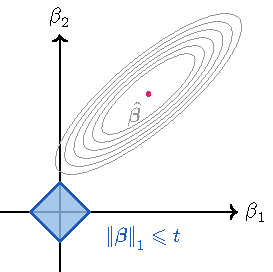
\includegraphics[height = 5cm]{figures/lasso.pdf}
    \end{subfigure}
    \begin{subfigure}[t]{0.48\linewidth}
        \centering
        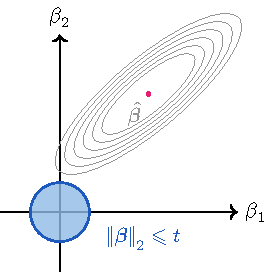
\includegraphics[height = 5cm]{figures/ridge.pdf}
    \end{subfigure}
    \caption{Comparison of constrain region \(R \leqslant t\) for LASSO (L1) and ridge (L2) regression.} % \label{}
\end{figure}
The sharp corners of the LASSO constraint region cause the level curves
of \(J\) to intersect the constraint region at the axes, leading to a
sparse solution. Because of it's constant radius, ridge regression tends
to produce a solution with small coefficients that are not necessarily
zero.
\section{Classification}
Classification is a supervised learning task that predicts classes of
categorical data. There are two main types of classification:
\begin{itemize}
    \item \textbf{Binary classification:} The response variable has two classes.
    \item \textbf{Multiclass classification:} The response variable has more than
          \(N\) classes.
\end{itemize}
\subsection{Classification Metrics}
In binary classification, the confusion matrix is a table that is used
to describe the performance of a classification model. It has the
following metrics:
\begin{figure}[H]
    \centering
    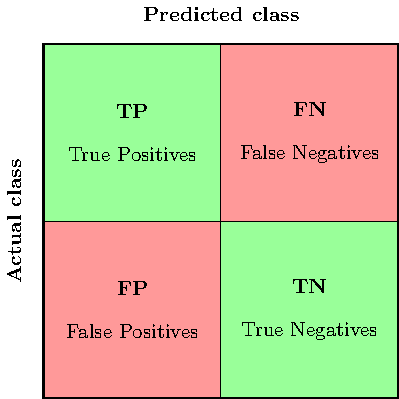
\includegraphics[height = 5cm]{figures/confusion_matrix.pdf}
    % \caption{} % \label{}
\end{figure}
The following metrics are used to assess the performance of binary
classification models.
\begin{table}[H]
    \centering
    \begin{tblr}
        {hlines,colspec={|Q[c,m]|Q[c,m]|Q[l,m]|}, rowsep=2ex, colsep=2ex}
        \textbf{Metric}    & \textbf{Formula}                                                                                                 & \textbf{Interpretation}               \\
        Accuracy           & \(\displaystyle\frac{\mathrm{TP} + \mathrm{TN}}{\mathrm{TP} + \mathrm{TN} + \mathrm{FP} + \mathrm{FN}}\)         & Overall performance of model          \\
        Precision          & \(\displaystyle\frac{\mathrm{TP}}{\mathrm{TP} + \mathrm{FP}} \)                                                  & Accuracy of positive predictions      \\
        Recall Sensitivity & \(\displaystyle\frac{\mathrm{TP}}{\mathrm{TP} + \mathrm{FN}}\)                                                   & Coverage of actual positive samples   \\
        Sensitivity        & \(\displaystyle\frac{\mathrm{TN}}{\mathrm{TN} + \mathrm{FP}}\)                                                   & Coverage of actual negative samples   \\
        F1 Score           & \(\displaystyle\frac{2 \times \mathrm{Precision} \times \mathrm{Recall}}{\mathrm{Precision} + \mathrm{Recall}}\) & Harmonic mean of precision and recall \\
    \end{tblr}
    % \caption{} % \label{}
\end{table}
Compared to accuracy, precision and recall provide a more detailed
analysis of how a model performs. Choosing the right metric depends on
what is important for a problem:
\begin{itemize}
    \item If we wish to minimise false negatives: Use recall.
    \item If we wish to minimise false positives: Use precision.
    \item For overall performance: Use accuracy.
\end{itemize}
These metrics can also be generalised to multiclass classification by
computing them for each class. Here we must consider datasets with class
imbalance, as the metrics may be biased towards the majority class.
\subsection{Support Vector Machines}
Support Vector Machines (SVM) are a supervised learning model used for
binary classification. The model works by finding a hyperplane that
separates classes with the maximum margin. Consider a dataset of \(n\)
points of the form:
\begin{equation*}
    \left\{ \left( \symbf{x}^{\left( i \right)},\: y^{\left( i \right)} \right) \right\}
\end{equation*}
where \(\symbf{x}^{\left( i \right)} \in \R^p\) is a \(p\)-dimensional
and \(y^{\left( i \right)} \in \left\{ -1,\: {+}1 \right\}\) indicates the
class of the \(i\)th point. We can model a \(p\)-dimensional
hyperplane by the equation:
\begin{equation*}
    \symbf{w}^\top \symbf{x} - b = 0
\end{equation*}
where \(\symbf{w} \in \R^p\) is a vector normal to the hyperplane and
\(b \in \R\) is the bias term. In this model, the distance between the
hyperplane and the origin is given by \(\abs*{b} / \norm*{\symbf{w}}\).
\subsubsection{Hard Margin SVM}
If a dataset is linearly separable, we can select two parallel
hyperplanes that separate the classes, such that the distance between
them is maximised.
% Given a normalised or standardised dataset, these hyperplanes can be
% described by
% \begin{equation*}
%     \symbf{w}^\top \symbf{x} - b = +1
% \end{equation*}
% such that all points on and above this hyperplane are of class \({+}1\), and
% \begin{equation*}
%     \symbf{w}^\top \symbf{x} - b = {-}1
% \end{equation*}
% such that all points on and below this hyperplane are of class \({-}1\).
We start by defining the \textbf{functional margin} of a point
\(\symbf{x}^{\left( i \right)}\) as
\begin{equation*}
    \hat{\gamma}^{\left( i \right)} = y^{\left( i \right)} \left( \symbf{w}^\top \symbf{x}^{\left( i \right)} - b \right)
\end{equation*}
and the \textbf{functional margin} of the optimal hyperplane as
\begin{equation*}
    \hat{\gamma} = \min_{i =  1,\:\dots,\: n} \hat{\gamma}^{\left( i \right)}
\end{equation*}
This value represents the \textbf{correctness} and \textbf{confidence}
of the classification of a point for a given hyperplane:
\begin{itemize}
    \item A hyperplane correctly classifies a point when
          \(\hat{\gamma}^{\left( i \right)} > 0\).
    \item A hyperplane confidentally classifies a point when
          \(\abs*{\hat{\gamma}^{\left( i \right)}} \gg 0\).
\end{itemize}
Using this definition, we also define the \textbf{geometric margin} of a
point \(\symbf{x}^{\left( i \right)}\), to allow us to compare the
confidence of points across different hyperplanes:
\begin{equation*}
    \gamma^{\left( i \right)} = \frac{\hat{\gamma}^{\left( i \right)}}{\norm*{\symbf{w}}}.
\end{equation*}
In a similar manner, the \textbf{geometric margin} of the optimal
hyperplane is defined:
\begin{equation*}
    \gamma = \frac{\hat{\gamma}}{\norm*{\symbf{w}}}
\end{equation*}
To understand why we define the functional margin in this way, consider
the points \(\symbf{x}_{{+}}\) that are classified as \({+}1\), and the
points \(\symbf{x}_{{-}}\) that are classified as \({-}1\). We wish to
constrain the two classes by the hyperplanes:
\begin{gather*}
    \symbf{w}^\top \symbf{x}_{{+}} - b \geqslant {+}\hat{\gamma} \\
    \symbf{w}^\top \symbf{x}_{{-}} - b \leqslant {-}\hat{\gamma}
\end{gather*}
If we multiply both equations by \(y\),
which for \(\symbf{x}_{{+}}\) is \({+}1\), and for \(\symbf{x}_{{-}}\)
is \({-}1\), we find:
\begin{gather*}
    \begin{cases}
        y \left( \symbf{w}^\top \symbf{x}_{{+}} - b \right) \geqslant \hat{\gamma} \\
        y \left( \symbf{w}^\top \symbf{x}_{{-}} - b \right) \geqslant \hat{\gamma}
    \end{cases}
    \\[1ex]
    \therefore\:\: y^{\left( i \right)} \left( \symbf{w}^\top \symbf{x}^{\left( i \right)} - b \right) \geqslant \hat{\gamma}.
\end{gather*}
We can then pose the following optimisation problem:
\begin{align*}
    \max_{\hat{\gamma},\: \symbf{w},\: b} \quad & \frac{\hat{\gamma}}{\norm*{\symbf{w}}}                                                                                                                                                          \\
    \text{subject to} \quad     & y^{\left( i \right)} \left( \symbf{w}^\top \symbf{x}^{\left( i \right)} - b \right) \geqslant \hat{\gamma}, \quad \forall i = 1,\: \dots,\: n
\end{align*}
This is a non-convex problem, as the objective function contains the
nonlinear term \(\norm*{\symbf{w}}\). If we impose the constraint
\begin{equation*}
    \hat{\gamma} = 1
\end{equation*}
and note that maximising \(\hat{\gamma} / \norm*{\symbf{w}} = 1 / \norm*{\symbf{w}}\)
is the same as minimising \(\norm*{\symbf{w}}^2\), we can solve the
equivalent problem:
\begin{align*}
    \min_{\symbf{w},\: b} \quad & \frac{1}{2}\norm*{\symbf{w}}^2                                                                                                                                                          \\
    \text{subject to} \quad     & y^{\left( i \right)} \left( \symbf{w}^\top \symbf{x}^{\left( i \right)} - b \right) \geqslant 1, \quad \forall i = 1,\: \dots,\: n.
\end{align*}
This is an optimisation problem with a convex quadratic objective
function and linear constraints whose solution gives us the
\textbf{optimal margin classifier}. The following figure shows a
geometric interpretation of the optimal margin classifier:
\begin{figure}[H]
    \centering
    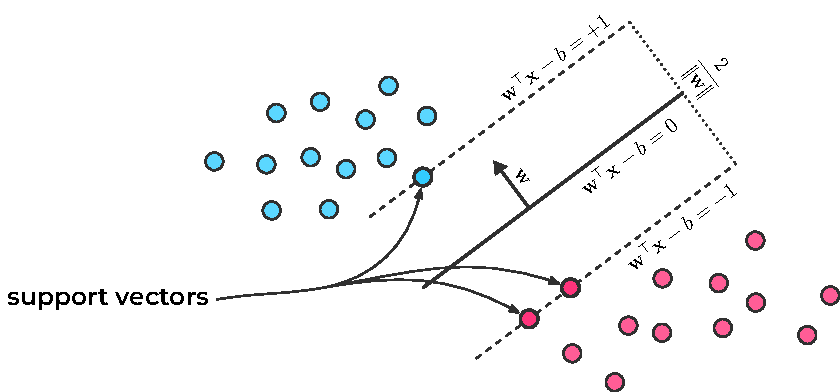
\includegraphics[width = \linewidth]{figures/hard_margin_svm.pdf}
    % \caption{} % \label{}
\end{figure}
The \textbf{decision boundary} is completely determined by the points
that lie nearest to it. These points are called \textbf{support vectors}.
\subsubsection{Soft Margin SVM}
The derivation of the SVM assumes that a dataset is linearly separable,
however we cannot guarantee this will always be the case. Additionally,
outliers in the dataset can cause the optimal margin classifier to
change dramatically, and produce a much smaller margin. To allow this
algorithm to work with non-linearly separable datasets, and also be
less sensitive to outliers, we will reformulate our optimisation
problem using a slack variable \(\xi^{\left( i \right)}\) for each
point \(\symbf{x}^{\left( i \right)}\):
\begin{align*}
    \min_{\symbf{w},\: b,\: \xi} \quad & \frac{1}{2}\norm*{\symbf{w}}^2 + C \sum_{i = 1}^n \xi^{\left( i \right)}                                                                                     \\
    \text{subject to} \quad             & y^{\left( i \right)} \left( \symbf{w}^\top \symbf{x}^{\left( i \right)} - b \right) \geqslant 1 - \xi^{\left( i \right)}, \quad \forall i = 1,\: \dots,\: n \\
                                        & \xi^{\left( i \right)} \geqslant 0, \quad \forall i = 1,\: \dots,\: n
\end{align*}
Modifying the first constraint now allows points to be misclassified
with a penalty \(C \xi^{\left( i \right)}\). The hyperparameter \(C\) is
a regularisation parameter that controls the trade-off between the
margin and the slack variables.
\begin{itemize}
    \item A small value of \(C\) will penalise misclassifications less,
         and result in a larger margin.
    \item A large value of \(C\) will penalise misclassifications more,
         and result in a smaller margin.
\end{itemize}
\(C = \infty\) is equivalent to the hard margin SVM.

\newpage
\begin{appendix}
    \section{Numerical Summaries of Data}\label{appendix:numerical-summaries}
    \subsection{Mean}
    The mean of a set of \(n\) observations \(\left( x^{\left( i
    \right)} \right)\) is given by:
    \begin{equation*}
        \bar{x} = \frac{1}{n} \sum_{i = 1}^n x^{\left( i \right)}
    \end{equation*}
    \subsection{Variance}
    The variance of a set of \(n\) observations \(\left( x^{\left( i
    \right)} \right)\) is given by:
    \begin{equation*}
        \sigma^2 = \frac{1}{n} \sum_{i = 1}^n {\left( x^{\left( i \right)} - \bar{x} \right)}^2
    \end{equation*}
    For a sample, the variance is given by:
    \begin{equation*}
        s^2 = \frac{1}{n - 1} \sum_{i = 1}^n {\left( x^{\left( i \right)} - \bar{x} \right)}^2
    \end{equation*}
    \subsection{Covariance}
    The covariance between two sets of \(n\) observations \(\left(
    x^{\left( i \right)} \right)\) and \(\left( y^{\left( i \right)}
    \right)\) is given by:
    \begin{equation*}
        \sigma_{xy} = \frac{1}{n} \sum_{i = 1}^n \left( x^{\left( i \right)} - \bar{x} \right) \left( y^{\left( i \right)} - \bar{y} \right)
    \end{equation*}
    For a sample, the covariance is given by:
    \begin{equation*}
        s_{xy} = \frac{1}{n - 1} \sum_{i = 1}^n \left( x^{\left( i \right)} - \bar{x} \right) \left( y^{\left( i \right)} - \bar{y} \right)
    \end{equation*}
\end{appendix}
\end{document}
